\documentclass{article}
\usepackage{blindtext}
\usepackage{graphicx}
\usepackage{subcaption}
\usepackage{hyperref}
\usepackage{float}
\usepackage{amsmath}
\usepackage{amssymb}
\usepackage[T1]{fontenc}
\usepackage[polish]{babel}
\usepackage[utf8]{inputenc}
\usepackage{multicol}
\usepackage{enumerate}
\usepackage{pbox}

\usepackage[margin=0.75in]{geometry}
\graphicspath{{./assets/}}
\title{BADANIE PROCESÓW ŁADOWANIA I ROZŁADOWANIA KONDENSATORA}



\begin{document}
\maketitle

\textbf{\underline{Cel ćwiczenia:}} wyznaczenie przebiegów ładowania i rozładowania kondensatora oraz
wyznaczenie stałej czasowej układów RC.
\\
\textbf{\underline{Zagadnienia:}} prawa Ohma i Kirchhoffa, dzielnik napięć, budowa i parametry kondensatora,
układ RC i jego zastosowania - całkowanie i różniczkowanie sygnału elektrycznego oraz filtrowanie.%

\subsubsection*{\textbf{\underline{Wprowadzenie:}}}

Kondensator służy do gromadzenia ładunku elektrycznego i jest układem dwóch odizolowanych elektrycznie przewodników. W najprostszym przypadku są to dwie jednakowe, równoległe względem siebie i odizolowane metalowe płyty. Przestrzeń między nimi jest wypełniona dielektrykiem, np. powietrzem. Symbol graficzny kondensatora „zwykłego" pokazano na rys. l a. Rysunek 1 b. pokazuje symbol kondensatora elektrolitycznego lub tantalowego. Ta grupa kondensatorów ma oznaczoną biegunowość elektrod - mylne ich połączenie może doprowadzić tło zniszczenia kondensatora. %

Ilość zgromadzonego na kondensatorze ładunku elektrycznego Q zależy od geometrii jego płyt, rodzaju zastosowanego dielektryka oraz przyłożonego do jego okładek napięcia U i jest opisana wzorem:

\begin{equation}
    \centering%
    \label{eq:intro}
    \mathbf{Q = C \cdot U}
\end{equation}

\begin{figure}[H]
    \centering
    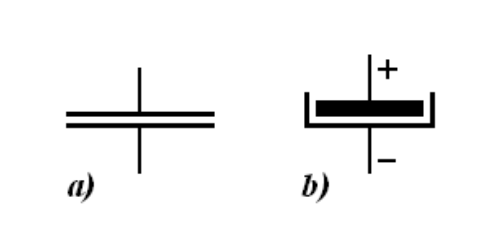
\includegraphics[width=0.5\linewidth]{capacitor_fig_1.png}%
    \label{fig:capacitor_fig}
    \caption{Symbole kondensatora: a) zwykłego, b) elektrolitycznego}
    \end{figure}


\subsubsection*{\textbf{\underline{Ładowanie kondensatora:}}}
Z praw Kirchhofia wynika, że napięcie zasilania $U_z$ równa się sumie napięć na oporniku $U_R = U_{AB}$ oraz na kondensatorze $U_C = U_{BD}$.

\begin{figure}[H]
    \centering
    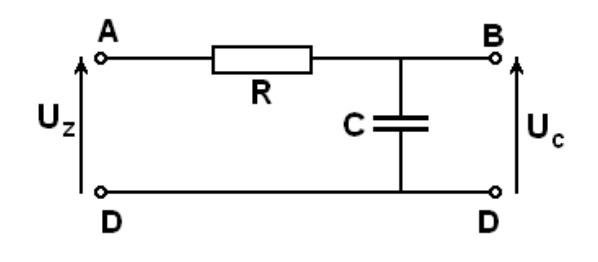
\includegraphics[width=0.5\linewidth]{capacitor_fig_2.png}%
    \label{fig:capacitor_charging_fig}
    \caption{Rozkład napięć w obwodzie zawierającym pojemność C i oporność R.}
    \end{figure}

Można więc zapisać, że:

\begin{equation}
    \centering%
    \label{eq:intro}
    \mathbf{U_R + U_C = U_Z}
\end{equation}

Z prawa Ohma oraz z definicji \eqref{fig:capacitor_fig} wynika, że

\begin{multicols}{2}
    \begin{equation}
        \nonumber
        \mathbf{U_R = I \cdot R}
    \end{equation}\break
    \begin{equation}
        \nonumber
        \mathbf{U_C = \frac{Q}{C}}
    \end{equation}
\end{multicols}


\subsection*{\textbf{Tok Postępowania:}}
\begin{enumerate}
    \item Placeholder
    \item {%
    Podłączyć wybrany przez prowadzącego ćwiczenia kondensator C (zacisk 6 połączyć z odpowiednim zaciskiem) oraz ustawić wskazaną wartość oporu R.
    Przygotować tabelę I.\par
    \begin{minipage}{\linewidth}
        \centering
        \begin{tabular}{|c | c | c | c|} 
            % https://tex.stackexchange.com/questions/2441/how-to-add-a-forced-line-break-inside-a-table-cell
            \hline
            \pbox{20cm}{\centering Opór \\ \textbf{R} \\ $\Omega$}  & \pbox{20cm}{\centering Czas \\ \textbf{t} \\ s} & \pbox{20cm}{\centering Napięcie na kondensatorze \\ \textbf{U} \\ V} & \pbox{20cm}{\centering Natężenie prądu \\ \textbf{I} \\ A} \\ [0.5ex] 
            \hline
                & & & & 
                & & & & 
                & & & & 
                & & & & 
                & & & & 
        \end{tabular}
    \end{minipage}
    }
\end{enumerate}

\end{document}


